\chapter{Recurrency}



%\ifpdf
%%    \graphicspath{{Chapter2/Figs/Raster/}{Chapter2/Figs/PDF/}{Chapter2/Figs/}}
%    \graphicspath{{D:/MyTemp/gitlocal/phd-thesis/text/chapter2/img/}}
%\else
%    \graphicspath{{Chapter2/Figs/Vector/}{Chapter2/Figs/}}
%\fi
%\section{Mixture settings PCCF}
%Take into account uncertainty of the parameters in PCCF by assigning prior probabilities to the set of possible values (Bayesian approach). 

\section{Motivation about concept drift}
% From recurrecny paper (commented)
Sensor generated data is available in a wide variety domains and applications such as traffic monitoring, personal health, production management, surveillance and many more, where predictive models are used for decision support.
As data is generated in a dynamic environment, it is unlikely for the data distribution to stay fixed over time.
Any significant changes need to be detected as soon as possible in order to update predictive models to respond to the most up-to-date situation.
%\section[Short title]
\section{On-line prediction of change points using recurrency information}
In the recurrency paper we describe temporal context incorporation.


%\section{Model hyper parameters update procedure}
%\section{On-line error correction using recurrency info (Dobro)}
\section{PCCF}
%............ COPIED INTO THESIS DESCRIPTION OF PCCF BEHAVIOR
Figure~\ref{fig:recprobs} illustrates behavior of the PCCF function~\ref{eq:confidencefunc} for  various parameters $\theta = (\mu, \sigma)$ of the Gaussian init-function (Eq.~\ref{eq:gaussianbelief}).%(Definition~\ref{def:gaussianbelief}).
Six cases are depicted with two PCCF functions calculated on each subplot for different ratios $\mu / \mu_0$ and $\sigma / \sigma_0$.

For all cases $\theta_0 = (\mu_0, \sigma_0)$ are parameters for the solid bold line (first PCCF).
For example in Case 1 average distance and standard deviations of the second PCCF (dashed line) are half of $\mu_0$ and $\sigma_0$ and we can see that limit $\mathcal{L}$ of the dashed line is higher.
In Case 2 $\mu = \mu_0 / 2$ but standard deviation is the same - dashed line converges to its limit very quickly.
In the third case second PCCF converges very slowly because $\sigma = \sigma_0 / 2$. It means that changes are more `recurrent' and we can predict longer with a good accuracy. In Case 5 we observe opposite case when $\sigma = \sigma_0 / 2$ and changes are not so strongly recurrent.
Thus, the figure illustrates that if we assume normal distribution of time intervals between changes then standard deviation is the main measure of degree of the `recurrence'.
It also can be seen that when time increases value of probabilities $\mathcal{P}_{t}(t)$ tends to some constant value:
\begin{equation}
\mathcal{L} = \lim_{t \to \infty} \mathcal{P} (t)
\label{eq:limit}
\end{equation}

\begin{figure*}[htb!]
\centering
%\includegraphics[width=0.8\textwidth]{"./Figs/recprobs.pdf"}
%\includegraphics[width=0.8\textwidth]{./chapter2/images/recprobs.pdf}
%\includegraphics[width=0.8\textwidth]{./chapter2/images/recprobs.pdf}
\includegraphics[width=0.8\textwidth]{pics/recprobs.pdf}
\caption{
Probabilities to observe recurrent change event (solid line) at every moment of time for various $\theta$.
}
\label{fig:recprobs}
\end{figure*}

Related ~\cite{Dries_AdaptiveDrift}, ~\cite{Gama_Kosina}

\section{Parameters uncertainty}
%\subsection{Uncertainty of the $\theta$ parameters of the PCCF function}
% PCCF $\mathbb{P}(\theta)$ 
%Probability distribution of $\theta$ is $p(\theta)$
Probability to observe change is given by PCCF function~\footnote{Using $p(y)=\int p(y, \theta) p(y|\theta) d \theta$ from~\cite{gelman2013bayesian}}
\[ 
p(c_i = t_j) = \int  G(c_i = t_j | \theta) F(\theta) d \theta
\] 
Where $\theta$ has a probability distribution
\[ \theta \sim F( \cdot | \gamma) \]

%................... COMMENTED .....................
% Uncomment this line, when you have siunitx package loaded.
%The SI Units for dynamic viscosity is \si{\newton\second\per\metre\squared}.
%\begin{figure}[htbp!]
%\centering
%\includegraphics[width=1.0\textwidth]{minion}
%\caption[Minion]{This is just a long figure caption for the minion in Despicable Me from Pixar}
%\label{fig:minion}
%\end{figure}
%
%\begin{landscape}
%
%\section*{Subplots}
%I can cite Wall-E (see Fig.~\ref{fig:WallE}) and Minions in despicable me (Fig.~\ref{fig:Minnion}) or I can cite the whole figure as Fig.~\ref{fig:animations}
%
%
%\begin{figure}
%  \centering
%  \begin{subfigure}[b]{0.3\textwidth}
%    \includegraphics[width=\textwidth]{TomandJerry}
%    \caption{Tom and Jerry}
%    \label{fig:TomJerry}
%  \end{subfigure}
%  \begin{subfigure}[b]{0.3\textwidth}
%    \includegraphics[width=\textwidth]{WallE}
%    \caption{Wall-E}
%    \label{fig:WallE}
%  \end{subfigure}
%  \begin{subfigure}[b]{0.3\textwidth}
%    \includegraphics[width=\textwidth]{minion}
%    \caption{Minions}
%    \label{fig:Minnion}
%  \end{subfigure}
%  \caption{Best Animations}
%  \label{fig:animations}
%\end{figure}
%
%
%\end{landscape}
